\subsection{Num}
\begin{frame}{Von Wörtern zu Zahlen}
	\begin{block}{Def.: $\text{Num}_k$}
		Zu einer Zahlenbasis $k$ definiere die Abbildung $\text{Num}_k : Z_k^* \to \nZ$ 

		\begin{align*}
			\text{Num}_k(\varepsilon) &= 0 \\
			\text{Num}_k(wx) &= k\cdot \text{Num}_k(w) + \text{num}_k(x) \text{ für alle } w\in Z_k^*, x\in Z_k\\[2ex]
			\text{wobei }\text{num}_k(x) &= x \text{ für alle } x \in \set{1,\dots,k-1}
		\end{align*}
	\end{block}
	\pause
	\begin{exampleblock}{Beispiel}
		\begin{align*}
			\text{Num}_2(11) &= 2\cdot \text{Num}_2(1) + \text{num}_2(1) \\
				&= 2\cdot 1 + 1 \\
				&= 3
		\end{align*}
	\end{exampleblock}
\end{frame}

\begin{frame}{Von Wörtern zu Zahlen}
	\begin{exampleblock}{Aufgabe: Berechne die Zahlenwerte von $321_4, B2_{16}$}
	\begin{align*}
	\text{Num}_4(321) &= \visible<2->{ 4\cdot \text{Num}_4(32) + \text{num}_4(1) \\
	&= 4\cdot \left( 4\cdot \text{Num}_4(3) + \text{num}_4(2) \right) + \text{num}_4(1) \\
	&= 4^2\cdot \text{num}_4(3) + 4 \cdot \text{num}_4(2) + \text{num}_4(1) \\
	&= 57 \\}
	\visible<3->{\text{Num}_{16}(B2) &=} \visible<4->{ 16 \cdot \text{Num}_{16}(B) + \text{num}_{16}(2) \\
	&= 16\cdot 11 + 2 \\
	&= 178}
	\end{align*}
	\end{exampleblock}
	\visible<5->{
	\begin{exampleblock}{Aufgabe}
		$\text{Num}_2(1), \text{ Num}_2(11), \text{ Num}_2(111), \text{ Num}_2(1111)$\\
		Was gilt allgemein für $\text{Num}_2(1^m)$ für $m \in \nN_0$?
	\end{exampleblock}}
\end{frame}

\subsection{mod und div}
\begin{frame}{Division und Modulo}
	\begin{block}{\div und \mod}
		$ x \div y$ ist die ganzzahlige Division von x durch y.\\
		$ x \mod y$ liefert den Rest dieser Division.
	\end{block} 
	\begin{block}{Beobachtung}
		$$ 0 \leq (x \mod y ) < y$$
	\end{block}
	\begin{block}{Lemma}
		$$ x = y \cdot (x \div y ) + \left( x \mod y \right)$$ 
	\end{block}
\end{frame}

\begin{frame}{Division und Modulo}
	\begin{exampleblock}{Beispiel}
		\begin{table}[h!]
			\begin{tabular}{c|cc}
				& $x\div y$ & $x\mod y$ \\ \hline
				$x=2,y=3$ \only<2-|handout:0>{&  0 & 2 } \only<1>{&&}\\
				$x=5 ,y=2$ \only<3-|handout:0>{ & 2 & 1 } \only<1-2>{&&} \\
				$x=8,y=2$ \only<4-|handout:0>{ & 4 & 0 } \only<1-3>{&&} \\	
			\end{tabular}
		\end{table}
	\end{exampleblock}
\end{frame}

\begin{frame}{Division und Modulo}
	\begin{exampleblock}{Aufgabe}
		Fülle die folgende Tabelle aus
		\begin{table}[h!]
		\begin{tabular}{c|cccccccccccc}
			$x$ & 0 & 1 & 2 & 3 & 4 & 5 & 6 & 7 & 8 & 9 & 10 & 11 \\ \hline
			$x\div 4 $ & \only<1>{ &&&&&&&&&&} \only<2-|handout:0>{0 & 0 & 0 & 0 & 1 & 1 & 1 & 1 & 2 & 2 & 2 & 2}\\
			$4\left( x\div 4\right) $ & \only<1-2>{&&&&&&&&&&} \only<3-|handout:0>{0&0&0&0&4&4&4&4&8&8&8&8}\\
			$x\mod 4$ & \only<1-3>{&&&&&&&&&&} \only<4-|handout:0>{0&1&2&3&0&1&2&3&0&1&2&3}
		\end{tabular}
		\end{table}
	\end{exampleblock}
\end{frame}

\subsection{Repr}
\begin{frame}{Repräsentation}
	\begin{block}{Def.: $Repr_k$}
		\begin{align*}
			Repr_k : \; &\nN_0 \to Z_k  \\
			n&\mapsto \begin{cases} repr_k(n) & \text{, falls } n<k \\
				Repr_k\left( n\div k \right) \cdot repr_k\left( n \mod 	k \right) & \text{, falls } n\geq k 
			\end{cases}\\
			\text{Wobei für alle } &x \in \nZ_k : \text{repr}_k(x) = x.
		\end{align*}
	\end{block}
	\pause
	\begin{exampleblock}{Aufgabe}
		Berechne folgende Darstellungen:\\
		$Repr_2(42) = \pause 101010$ \\
		$Repr_4(42) = \pause 222$ \\
		$Repr_8(42) = \pause 52$ \\
		$Repr_{16}(42) = \pause 2A$
	\end{exampleblock}
\end{frame}

% \begin{frame}{Beispiel: Lösung}
% 	\begin{align*}
% 		Repr_8(42) &= Repr_8(42 \div 8) \cdot repr_8(42 \mod 8) \\
% 		&= Repr_8(5) \cdot repr_8(2)\\
% 		&= repr_8(5) \cdot 2\\
% 		&= 5 \cdot 2\\
% 		&= 52_8
% 	\end{align*}
% \end{frame}

\begin{frame}{Repräsentation}
	\begin{block}{Korrolar}
		$Repr_k(n)$ ist das kürzeste Wort $w\in Z_k^\ast$ mit $Num_k(w)=n$, also 
		$$ Num_k\left( Repr_k(n)\right) = n $$
	\end{block}

	\begin{alertblock}{Anmerkung}
		Im Allgemeinen  $Repr_k\left(Num_k(w)\right) \neq w $, da überflüssige Nullen wegfallen.
	\end{alertblock}
	
	\Stephan{
	\begin{exampleblock}{Schaubild}
		s. Tafel
	\end{exampleblock}
	}
	%TODO
	% \begin{exampleblock}{Zusammenhang}
	% 	\begin{tikzpicture}[
 %    		node distance=2mm,
 %    		>=stealth, auto,
	% 		every state/.style={draw=none, inner sep=0pt}
 %                		]

	% 			\node[state] (q1) {Dezimaldarstellung};
	% 			\node[state] (q2) [above right=of q1] {$\text{Repr}_k$};
	% 			\node[state] (q3) [below right=of q2] {k-äre Darstellung};
	% 			\node[state] (q4) [below right=of q1] {$\text{Num}_k$};

 %    		\begin{scope}[bend left]%
	% 	\path[->]   (q1) edge node {c} (q2)
 %            		(q2) edge node {c} (q3)
 %            		(q3) edge node {c} (q4)
 %            		(q4) edge node {c} (q1);
 %    		\end{scope}
	% 	\end{tikzpicture}
	% \end{exampleblock}	 
\end{frame}

\subsection{Zweierkomplement}
\begin{frame}{Ein asymetrischer Zahlenbereich}
	\[
	\nK_{\ell} := \{ x\in \nZ\mid -2^{\ell-1} \leq x \leq 2^{\ell-1} -1 \} \;.
	\]
	\\[0.2cm]
	
	\begin{figure}
		\centering
		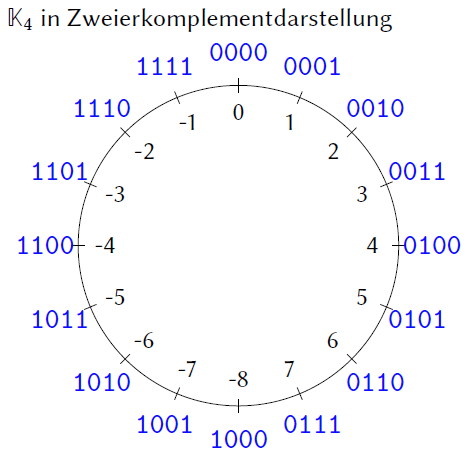
\includegraphics[scale=0.35]{../topics/codierung/ZK_K4}
	\end{figure}

	\begin{exampleblock}{Frage}
		Wie sieht $\nK_5$ aus?
	\end{exampleblock}
\end{frame}

\begin{frame}{Zweierkomplement} % TODO nötig?
    Das Zweierkomplement ist eine Möglichkeit, negative Zahlen binär darzustellen. Im Vergleich zu anderen Darstellungsarten ist es besonders vorteilhaft bei arithmetischen Rechnungen mit Hardware \textit{(mehr dazu in Technischer Informatik)}.
\end{frame}

\begin{frame}{Zweierkomplement}
	\begin{block}{Def.: $\text{Zkpl}_\ell$}
		Die Zweierkomplementdarstellung $ \text{Zkpl}_\ell: \nK \to \set{\texttt{0}, \texttt{1}}^\ell$ der Länge $\ell$:
		$$\text{Zkpl}_\ell(x) = \begin{cases} 0 \text{bin}_{l-1}(x) & \text{falls } x \geq 0 \\ 1 \text{bin}_{l-1}(2^{l-1}+x) & \text{falls } x < 0\end{cases}$$
		Äquivalent:
		$$\text{Zkpl}_\ell(x) = \begin{cases} \text{bin}_{l}(x) & \text{, falls } x \geq 0 \\ \text{bin}_{l}(2^{l}+x) & \text{, falls } x < 0\end{cases}$$
		wobei
		\[
			\text{bin} \colon \nZ_{2^{\ell}} \to \{\texttt{0},\texttt{1}\}^{\ell}, n \mapsto \texttt{0}^{\ell- |\text{Repr}_2(n)|} \text{Repr}_2(n) 
		\]
	\end{block}
\end{frame}
\subsection{Trick}
\begin{frame}{Zweierkomplement}
	\begin{exampleblock}{Ein Trick}
		Zum ``intuitiven'' Berechnen des Zweierkomplement können wir so vorgehen (für $x < 0$):
		\begin{enumerate}
			\item Binärdarstellung von $|x|$ berechnen: $\text{Repr}_2(|x|)$
			\item Mit führenden Nullen auffüllen bis zur Länge $\ell$
			\item Alle binären Ziffern negieren
			\item 1 addieren
		\end{enumerate}
	\end{exampleblock}

	\begin{exampleblock}{Beispiel}
		$$\text{Zkpl}_4(-2): 2 \rightarrow 10 \rightarrow 0010 \rightarrow 1101 \rightarrow 1110 = \text{Zkpl}_4(-2)$$
	\end{exampleblock}
\end{frame}
\subsection{Aufgabe}
\begin{frame}{Zweierkomplement}
	\begin{exampleblock}{Aufgaben}
	Berechne
		\begin{itemize}
			\item $\text{Zkpl}_5(0) \only<2->{= 00000}$ \\
			\item $\text{Zkpl}_5(2) \only<3->{= 00010}$ \\
			\item $\text{Zkpl}_5(15) \only<4->{= 01111}$ \\
			\item $\text{Zkpl}_5(-1) \only<5->{= 11111} $\\
			\item $\text{Zkpl}_5(-6) \only<6->{= 11010} $\\
			\item $\text{Zkpl}_5(-16) \only<7->{= 10000}$
		\end{itemize}
	\end{exampleblock}
\end{frame}

\begin{frame}{Darstellung von Zahlen}
    \begin{exampleblock}{Aufgabe}
    	Es seien die Wörter $u := \texttt{10010}, v := \texttt{01011}$ aus $Z_2^*$.
    	\begin{enumerate}
     		\item Gib die Dezimaldarstellung an, die $u$ und $v$ als Binärdarstellung haben. Gib die Binärdarstellung von $u+v=:w \in Z_2^*$ an.
    		\item Gib die Zweierkomplementdarstellung der Zahlen $u, v, w$ an.
    		\item Ist $w$ die Zweierkomplementdarstellung der Summe der Zahlen mit den Zweierkomplementdarstellungen $u$ und $v$?
  		\end{enumerate}
    \end{exampleblock}
    \pause
    \begin{block}{Lösung}
    	\begin{enumerate}
     		\item $\text{Num}_2(u)=18, \text{Num}_2(v)=11, \text{Num}_2(w) = \text{Num}_2(u)+\text{Num}_2(v)=29, w=\texttt{11101}$
    		\pause \item $\text{Num}_{Zkpl}(u)=-14, \text{Num}_{Zkpl}(v)=\text{Num}_2(v)=11, \text{Num}_{Zkpl}(w)=-3$
    		\pause \item Ja, denn $-14+11=-3$.
  		\end{enumerate}
    \end{block}
\end{frame}


% \begin{frame}{ZK: Einfache Berechnung}
% 	Die einzelnen Schritte können wir auch formal angeben:\\
% 	(Wir operieren jeweils auf Wörtern aus $\{0, 1\}^* = Z_2^*$) \\[0.5em]
% 	1. Binärdarstellung von $\setsize{x}$ berechnen: $Repr_2(\setsize{\cdot})$ \\
% 	2. Mit führenden Nullen auffüllen bis zur Länge $\ell$\\ \pause
% 	\begin{align*}
% 		Fill_\ell : Z_2^m &\to Z_2^\ell \qquad (m \le \ell) \\ \visible<3-> {
% 		w &\mapsto \begin{cases}
% 		0^\ell & w = \varepsilon \\
% 		Fill_{\ell-1}(w') \cdot \mu & w = w' \cdot \mu, w' \in Z_2^*, \mu \in Z_2
% 		\end{cases} \\
% 		&\text{oder deutlich einfacher} \\
% 		w &\mapsto \begin{cases}
% 		w & \setsize{w} = \ell \\
% 		Fill_\ell(0w) & \text{sonst}
% 		\end{cases} \\
% 	}
% 	\end{align*}
% 	\pause[4] 3. / 4. Analog %TODO
% \end{frame}